\clearpage
\section{Umsetzung}
\subsection{Benutzerführung}
Die Applikation wurde so als Konsolenapplikation angelegt, dass alle Module auch einzeln verwendet werden können. Für Enduser wurde jedoch im \lstinline$starter.py$ ein Konsolen-gesteuerter Workflow implementiert.

\begin{enumerate}
	\item Titel für die Suche muss eingegeben werden
	\item Der Benutzer wird gefragt, ob er bereits vorhandene Twitterdaten analysieren will oder ob er neue Twitterdaten über das API herunterladen möchte.
	\begin{enumerate}
		\item Wenn der Benutzer neue Twitterdaten laden möchte wird er nach Schlüsselwörtern gefragt
		\item Dem Benutzer werden die eingegebenen Schlüsselwörter nochmals angezeigt und er muss bestätigen damit das API angestossen wird
		\item Die Daten werden heruntergeladen und im File \lstinline$keyword1_keyword2_...keywordn_raw_search_timestamp.txt$ abgelegt. Der Filepfad wird zurückgegeben.
	\end{enumerate}
	\item Wenn der Benutzer vorhandene Twitterdaten analysieren möchte, muss er den Pfad zum Twitterdatenfile angeben
	\item Der Benutzer bestätigt, dass er die Twitter Datenanalyse für die gegebenen Tweets starten möchte
	\item Das Programm analysiert die Daten, erstellt die Plots und ein Logfile mit Resultaten
\end{enumerate}

Live sieht dies wie in Abbildung \ref{fig:benutzerfuehrung} aus.

\begin{figure}[h]
  \centering
  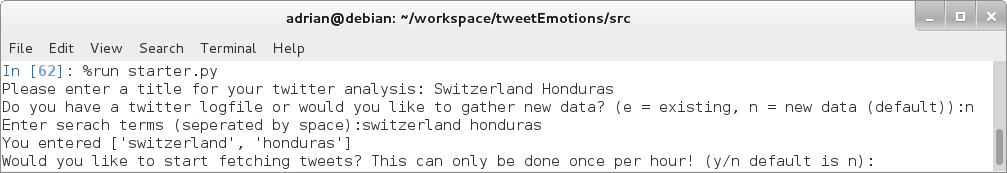
\includegraphics[width=0.8\textwidth]{images/benutzerfuehrung.png}
  \caption[Benutzerführung]{Benutzerführung}
  \label{fig:benutzerfuehrung}
\end{figure}

\subsubsection{Verwendete bzw. Eingebundene Ressourcen}
\begin{table}[H]
\begin{center}
\begin{tabular}{|l|l|}
	\hline
	\lstinline$starter.py$ & Enthält den Code der Benutzerführung \\ \hline
	\lstinline$gather_twitterdata.py$ & Enthält sowohl die Benutzerführung als auch die \\
	& Methoden zum herunterladen der Tweets \\ \hline
	\lstinline$analyse_twitterdata.py$ & Wird mit MPI angestossen um die Daten zu analysieren \\ \hline
\end{tabular}
\caption{Verwendete Ressourcen: Benutzerführung}
\end{center}
\end{table}


\subsection{Twitterdaten Sammeln}
Wie bereits im Kapitel \ref{subsec:grundlagentwitter} beschrieben wurde zum Herunterladen der Tweets das Package TwitterSearch von Christian Koepp\cite{twittersearch} verwendet.

Im File \lstinline$gather_twitterdata.py$ werden - geführt - Twitterdaten heruntergeladen. Das heisst, der Benutzer wird nach Schlüsselwörtern gefragt, darauf aufmerksam gemacht, dass nach einem Twitter API Call das Interface für eine weile blockiert sein wird, er muss bestätigen, dass er den Interface Call wirklich mit den von ihm eingegebenen Parametern anstossen will und zum Schluss wird ihm der Dateiname des Twitter Logs angezeigt.

Das schreiben der Tweets läuft wie folgt ab:
\begin{enumerate}
	\item Tweet und Benutzer auslesen
	\item Zeilenumbrüche im Tweet durch Leerschläge ersetzten
	\item String im Format \lstinline$user \\t tweet \\n$ zusammensetzen
	\item String ins File schreiben 
\end{enumerate}

Wie im Listing \ref{lst:twitterlogformat} ersichtlich, führt dieser Schreibvorgang zu Files bei welchen auf jeder Zeile ein Benutzername und ein Tweet steht. Innerhalb jeder Zeile sind Benutzernamen und Tweets mit einem Tabulator voneinander getrennt.

\begin{lstlisting}[showtabs=true, caption={Twitter Logfile Format)}, label={lst:twitterlogformat}]
UrbanRadio254	Do you think Sepp Blatter is too old to lead FIFA? #UrbanKickOff
AlanMcnee1	I am thinking of running as head of FIFA. I'm going tae be the new Sepp Blatter. 'Sepp Bladdered.'
blunt_waves	Sepp #Blatter is as corrupt as most of the rulers we have in #Africa. #FIFA.
\end{lstlisting}

\subsubsection{Verwendete bzw. Eingebundene Ressourcen}
\begin{table}[H]
\begin{center}
\begin{tabular}{|l|l|}
	\hline
	\lstinline$gather_twitterdata.py$ & Enthält sowohl die Benutzerführung als auch die\\
	& Methoden zum herunterladen der Tweets \\ \hline
	\lstinline$TwitterSearch$ & Library zum ansteuern der Twitter API\\ \hline
\end{tabular}
\caption{Verwendete Ressourcen: Benutzerführung}
\end{center}
\end{table}

\subsection{Algorithmen zur Erkennung der Gefühlslage in Texten}
\subsubsection{Emoticons}
Als Grundlage für den Emoticon Algorithmus wurden als erstes, wie im Listing \ref{lst:emoticonlisting} ersichtlich, Emoticons von den verschiedenen Quellen \cite{emoticons1}\cite{emoticons2}\cite{emoticons3}\cite{emoticons4} zusammengetragen und in die drei Gruppen positiv, negativ und neutral aufgeteilt.

\begin{lstlisting}[language=Python, caption={Emoticon Arrays}, label={lst:emoticonlisting}]
positive = [u'\u263B', u'\263A', u':)', u':D', u':-D', u':]', u':}', u':o)', u':o]', u':o}', u':-]', u':-)', u':-}', u'=)', u'=]', u'=}', u'=^]', u'=^)', u'=^}', u':B', u':-D', u':-B', u':^D', u':^B', u'=B', u'=^B', u'=^D', u':\'), u':\']', u':\'}', u'<3', u'^.^', u'^-^', u'^_^', u'^^', u':*', u'=*', u':-*', u';)', u';]', u';}', u':-p', u':-P', u':-b', u':^p', u':^P', u':^b', u'=P', u'=p', u'/o/', u':P', u':p', u':b', u'=b', u'=^p', u'=^P', u'=^b', u'\o/']
negative = [u'\u2639',u'D:', u'D=', u'D-:', u'D^:', u'D^=', u':(', u':[', u':{', u':o(', u':o[', u':^(', u':^[', u':^{', u'=^(', u'=^{', u'>=(', u'>=[', u'>={', u'>=(', u'>:-{', u'>:-[', u'>:-(', u'>=^[', u'>:-(', u':-[', u':-(', u'=(', u'=[', u'={', u'=^[', u'>:-=(', u'>=[', u'>=^(', u'=\\', u':\\', u'=/', u'=$', u'o.O', u'O_o', u'Oo', u':$:-{', u'>:-{', u'>=^{', u':o{']
neutral = [u':|', u'=|', u':-|', u'>.<', u'><', u'>_<', u':o', u':0', u'=O', u':@', u'=@', u':^o', u':^@', u'-.-', u'-_-', u':x', u'=X', u':-x', u':-@', u':-#', u':^x']
\end{lstlisting}

Um einen Tweet zu analysieren, wird nun mithilfe der Python Methode \lstinline$string.count(substring)$ gezählt wie viele positive, negative und neutrale Emoticons im Tweet vorkommen. Der Rückgabewert bestimmt sich dann wie folgt:

\begin{itemize}
	\item positive - Wenn mehr positive als negative Emoticons vorkommen
	\item negative - Wenn mehr negative als positive Emoticons vorkommen
	\item neutral - Wenn gleich viele positive und negative Emoticons vorkommen oder nur neutrale Emoticons vorhanden sind
	\item unsure - Wenn keine Emoticons gefunden wurden
\end{itemize} 

Umgesetzt wurde das Ganze im File \lstinline$emoticon_algorithm.py$.

\subsubsection{SentiWordNet}

\subsubsection{SenticNet}

\subsubsection{SASA}

\subsubsection{NLTK naive Bayes}

\subsection{Parallelisierung}